\documentclass[12pt]{article}

% Packages
\usepackage[utf8]{inputenc}
\usepackage[T1]{fontenc}
\usepackage{amsmath, amssymb, amsfonts}
\usepackage{graphicx}
\usepackage{float}
\usepackage{setspace}
\usepackage{enumitem}
\usepackage{parskip}
\usepackage{xcolor}
\usepackage{siunitx}
\usepackage{hyperref}
\usepackage{geometry}
\usepackage{booktabs}
\usepackage{caption}
\geometry{margin=1in}

% Web-article formatting
\setcounter{secnumdepth}{0}
\setlength{\parindent}{0pt}
\setlength{\parskip}{0.8em}
\renewcommand{\baselinestretch}{1.08}

% Custom colors and hyperlinks
\definecolor{linkcolor}{RGB}{0, 90, 160}
\definecolor{softblue}{RGB}{237, 246, 252}
\definecolor{softgray}{RGB}{245, 245, 245}
\definecolor{darkgray}{RGB}{70, 70, 70}
\hypersetup{
    colorlinks=true,
    linkcolor=linkcolor,
    urlcolor=linkcolor,
    citecolor=linkcolor
}

\begin{document}

\begin{center}
    {\Huge\bfseries Can Premier League Clubs Buy Points?}\par
    \vspace{0.35em}
    {\large Sam Reiner, James Duong, and Jonathan Pipping-Gam\'on}\par
    {\small Wharton Sports Analytics \& Business Initiative \; | \; \today}\par
\end{center}

\vspace{0.5em}
\hrule
\vspace{1.0em}

\section{The Premier League's Two Tables}

Every Premier League season has the table everyone watches: points, wins, losses, goal difference, survival, Europe, and the title. But beneath that table sits another one: the wage table.

It does not get updated on Match of the Day. It does not decide who lifts the trophy in May. But it helps explain why some clubs spend most seasons chasing Champions League places while others spend most seasons trying to stay up.

The logic is straightforward. Clubs with larger wage bills can compete for better players, retain stars for longer, and absorb mistakes that smaller clubs cannot afford. Over a 38-match season, that financial advantage should show up on the pitch.

So the obvious question is simple: does payroll buy points?

At first, the answer appears to be yes. Manchester City, Liverpool, Arsenal, Chelsea, Manchester United, and Tottenham usually spend more than the rest of the league, and they usually finish near the top. Lower-spending clubs tend to live closer to the relegation line. The relationship looks almost too obvious to analyze.

But that is not the question an owner, sporting director, or investor actually needs answered. The important question is not whether rich clubs are better than poor clubs. Everyone already knows that.

The sharper question is this: when a club increases its own wage bill, does it actually get better?

That is the question this analysis tries to answer.

\section{How We Measure Spending}

We use Premier League club-season data from 2013--14 through 2024--25 from FBRef. For each club-season, the data include the club, season, league points, and annual player wage bill in pounds.

Because wages rise over time across the league, raw wage bills are not directly comparable across seasons. A \pounds{}100 million payroll means something different in 2013--14 than it does in 2024--25.

To account for that, we scale each club's payroll by the league median in that season:
\[
W_{it}=\frac{\text{Payroll}_{it}}{\text{MedianPayroll}_t}.
\]

A value of \(W_{it}=1\) means the club spent exactly the league median. A value of \(W_{it}=2\) means the club spent twice the league median. A value of \(W_{it}=0.5\) means the club spent half the league median.

This scaling gives the estimates a useful interpretation: the expected change in league points associated with increasing payroll by one league-median wage bill.

For the 2024--25 season, the league-median wage bill is approximately \pounds{}70.6 million. We use that figure when translating model estimates into pounds per expected point.

\section{The First Look: Money and Points Move Together}

Start with the broadest version of the question: across the whole league, do higher-payroll teams earn more points?

Yes. Very clearly.

A pooled regression of points on relative wage bill suggests that increasing payroll by one league-median wage bill is associated with about 18.20 additional points. In 2024--25 money, that works out to roughly \pounds{}3.88 million per expected point.

\begin{figure}[H]
\centering
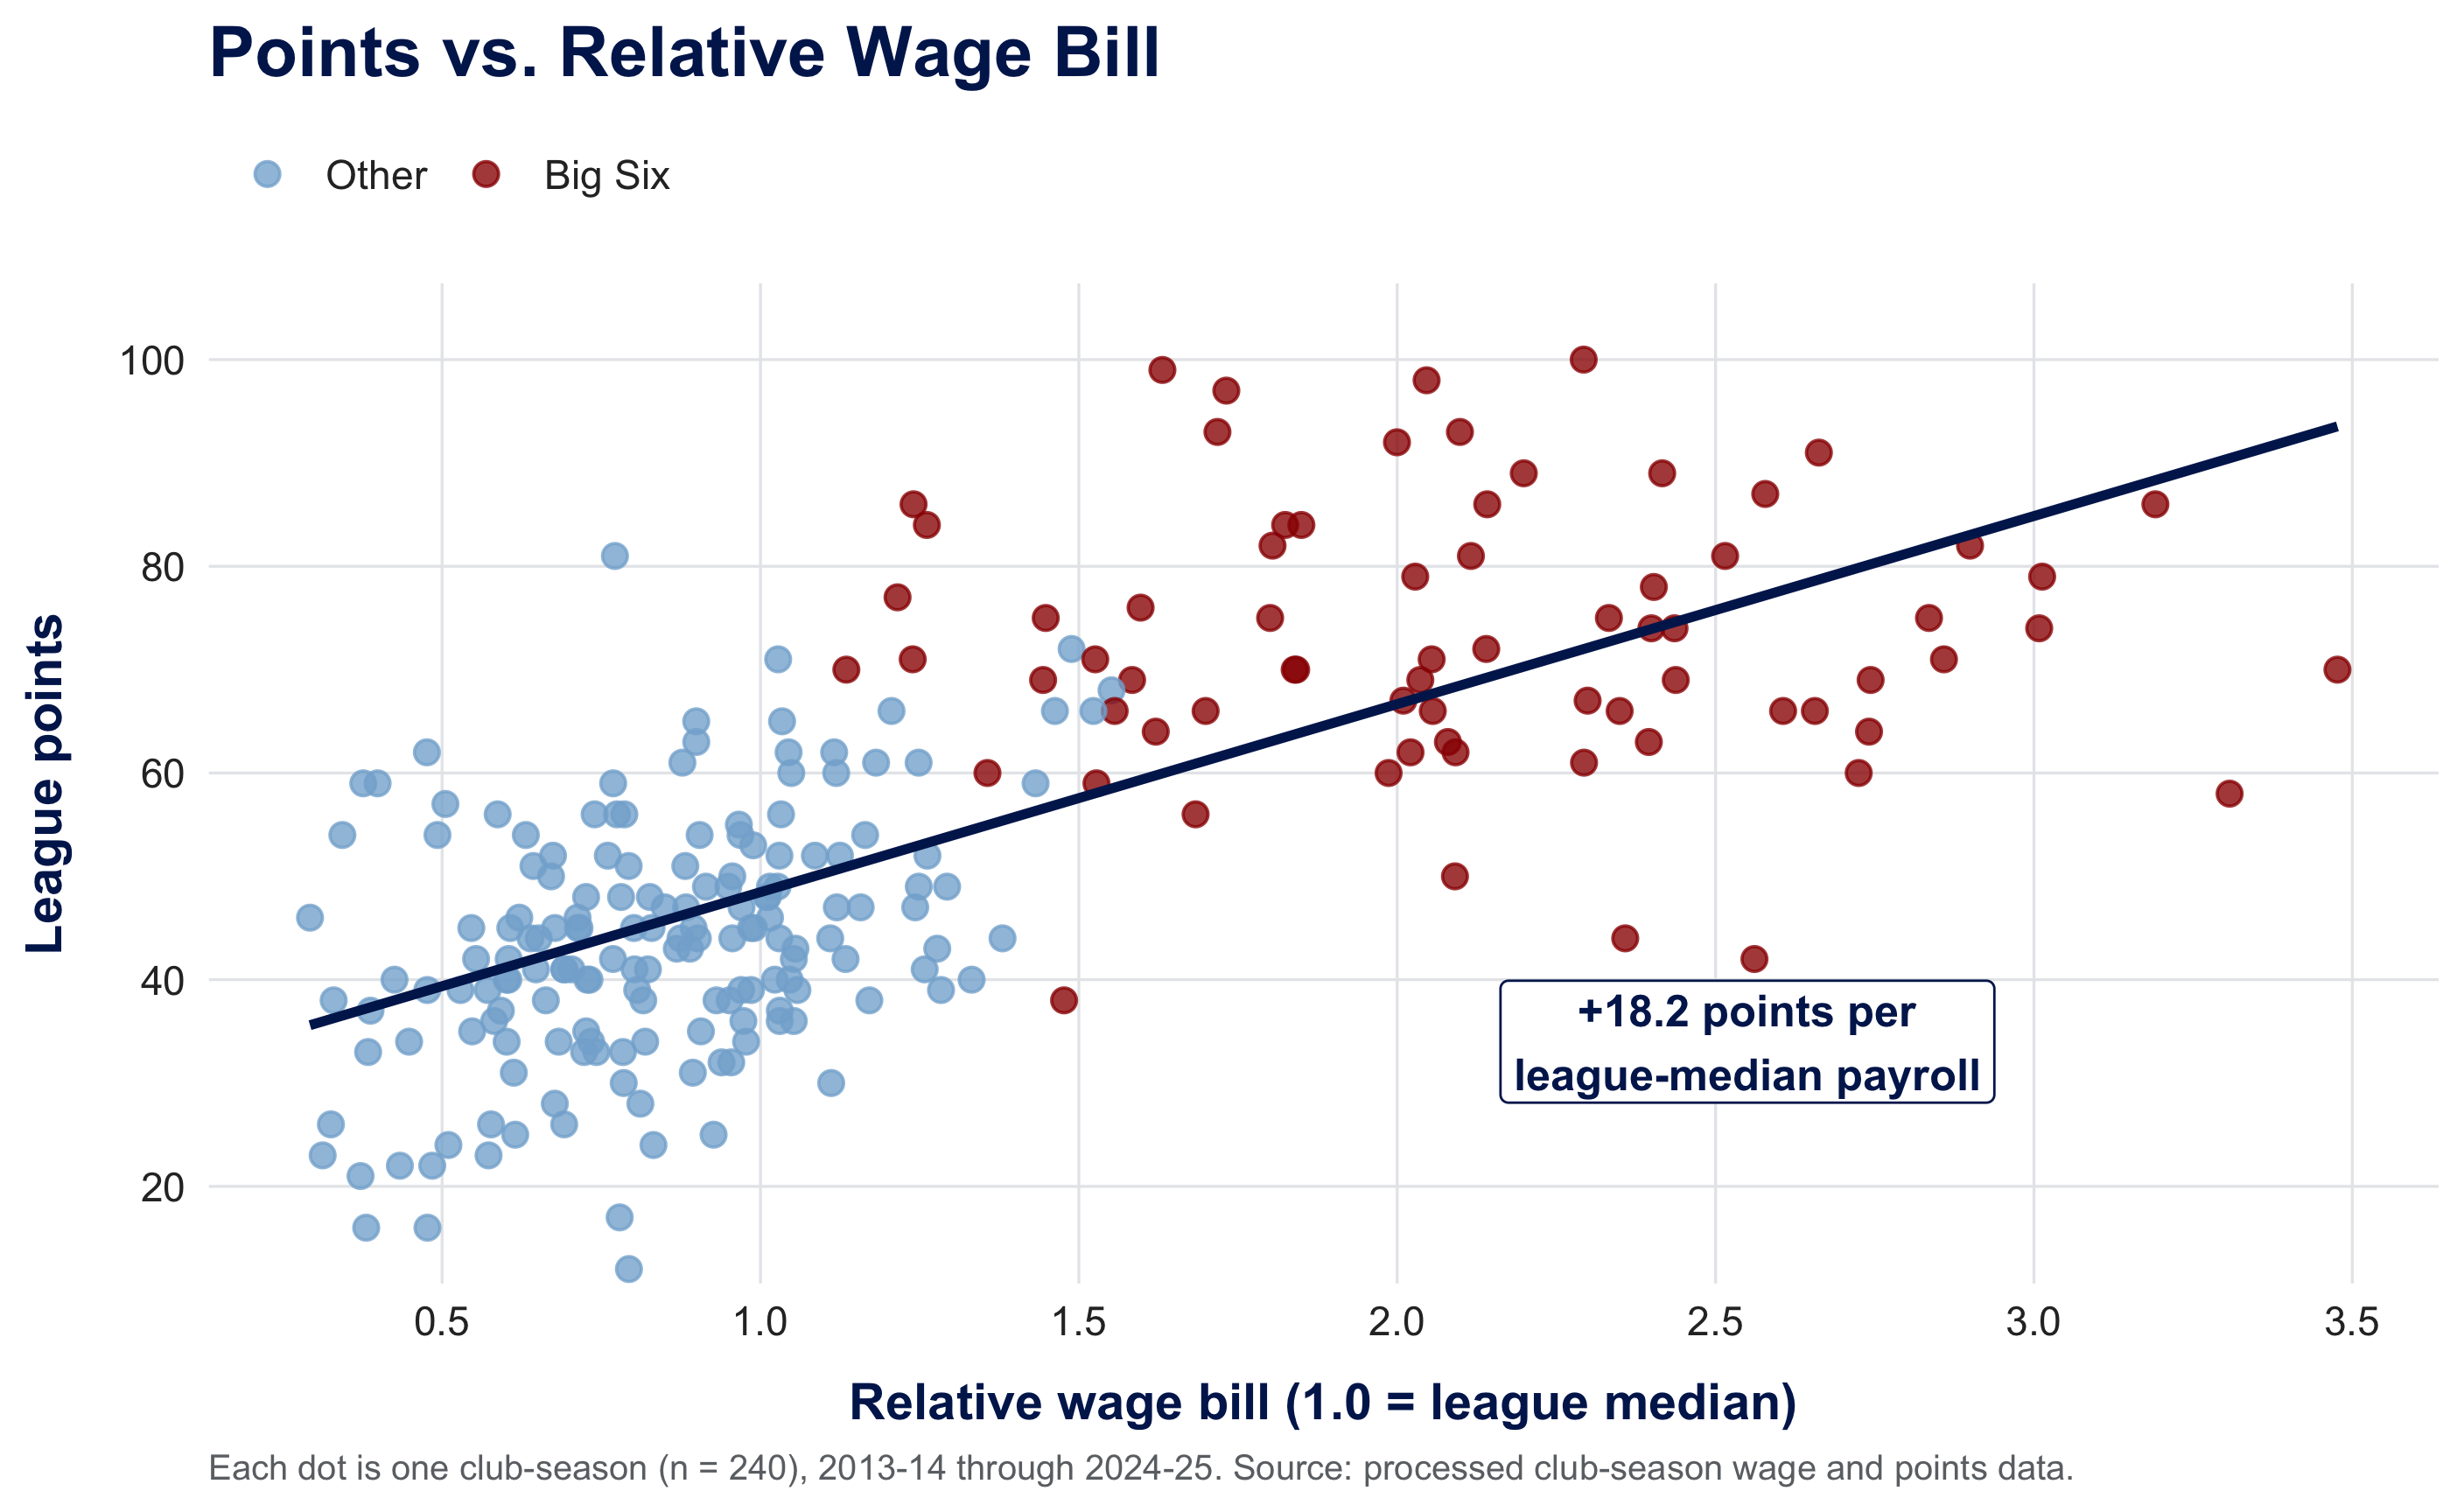
\includegraphics[width=\textwidth]{01_overall_relationship.png}
\caption*{\textbf{High-payroll clubs tend to earn more points.} Each dot is one club-season (\(n=240\)). The pooled line shows the strong league-wide association between relative payroll and points before accounting for persistent differences across clubs.}
\end{figure}

This is the version of the story most fans would expect. Spend more, get better players, earn more points.

But this first look answers the easiest question, not the most useful one. It tells us that richer clubs tend to be stronger. It does not tell us whether additional spending helps a given club improve.

\section{The Problem With Comparing Clubs to Each Other}

A Premier League wage bill is not just a spending decision. It is also a status signal.

The biggest clubs do not simply spend more because they choose to. They spend more because they have larger fan bases, stronger commercial revenue, deeper squads, Champions League appeal, better recruiting power, and long histories of attracting elite players.

That means the raw payroll-points relationship mixes together two different forces:

\begin{itemize}[leftmargin=*]
    \item \textbf{Structural club strength:} bigger clubs spend more and usually win more.
    \item \textbf{Marginal wage investment:} a club raises payroll and hopes to improve.
\end{itemize}

For decision-makers, the second force matters more. An owner cannot simply choose to become Liverpool or Manchester City overnight. But an owner can approve a larger wage bill.

So we need to ask a different question: what happens when we compare clubs to themselves?

\section{The Story Changes Within Clubs}

To isolate within-club changes, we estimate a model with club fixed effects:
\[
\text{Points}_{it}=\alpha_i+\beta W_{it}+\varepsilon_{it}.
\]

In plain English, this gives each club its own baseline. Instead of asking whether high-payroll clubs earn more points than low-payroll clubs, the model asks whether a club earns more points in seasons when it spends more than its own usual level.

That changes the result substantially.

Once club fixed effects are included, the payroll coefficient falls from 18.20 to 3.69 and is not statistically significant (\(p=0.280\)). In 2024--25 money, the point estimate would imply about \pounds{}19.16 million per expected point, but that figure should not be treated as a reliable decision rule because the estimate is imprecise.

\begin{figure}[H]
\centering
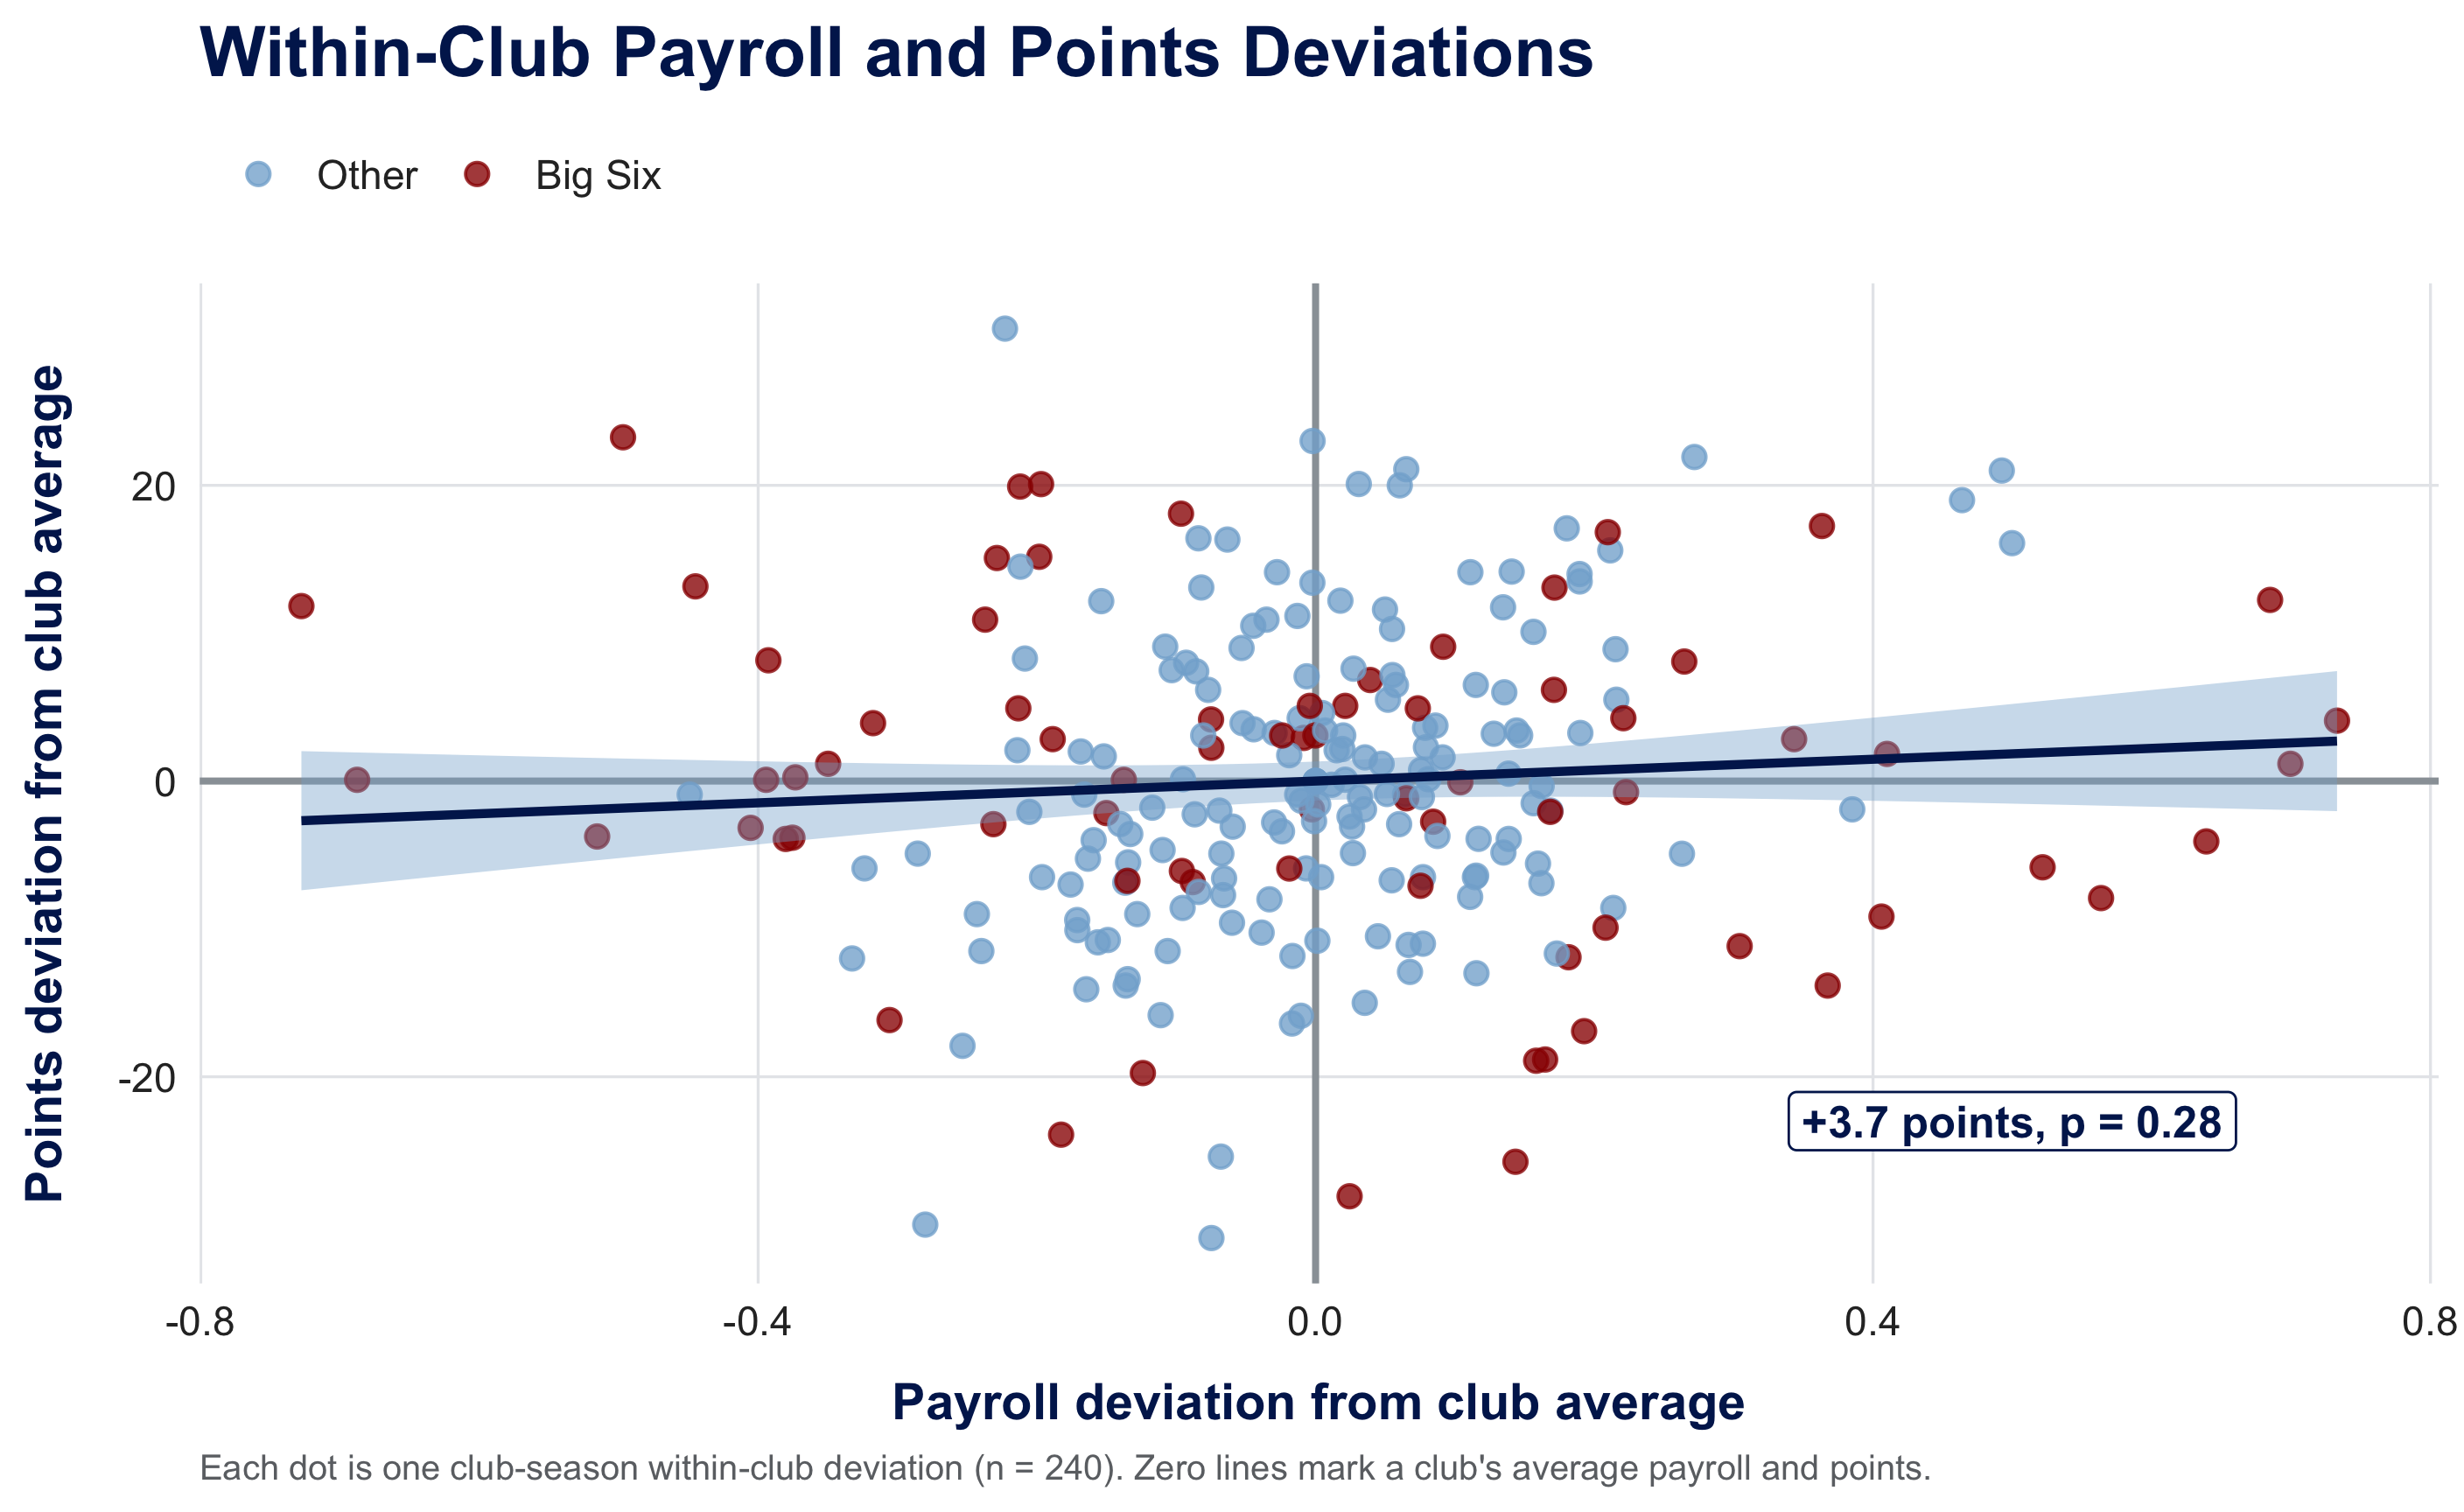
\includegraphics[width=\textwidth]{02_team_effects.png}
\caption*{\textbf{The relationship weakens within clubs.} Each dot is a within-club deviation from that club's average payroll and points (\(n=240\)). The fitted line is shallow and imprecise, and the zero lines mark each club's average.}
\end{figure}

This is where the simple spending story breaks down. Payroll is very good at identifying which clubs tend to be strong. It is much less reliable, on average, at predicting whether a club improves when it spends more than usual.

But the average within-club result may still be hiding an important divide. The Premier League is not one labor market. It is closer to two.

\section{The Premier League Is Not One Spending Market}

There is a structural divide between the Big Six and everyone else.

Arsenal, Chelsea, Liverpool, Manchester City, Manchester United, and Tottenham Hotspur operate in a different financial universe from most of the league. They rarely appear outside the top tier of the wage distribution. Most other clubs rarely get close to Big Six spending levels.

That matters because the return to payroll may depend on where a club starts.

For a lower- or middle-spending club, a higher wage bill can open access to a different class of player. It can help turn a relegation-caliber squad into a stable one, or a mid-table squad into a European contender.

For a Big Six club, the problem is different. These clubs are already shopping near the top of the player market. Additional payroll may go toward retaining stars, winning bidding wars for scarce elite players, or maintaining an already-expensive squad rather than meaningfully raising its quality.

The same pound may therefore mean very different things depending on the club spending it.

So we split the league into two groups: Big Six and non--Big-Six.

\section{Where Payroll Still Has Room to Work}

We estimate a model with club fixed effects and allow the payroll slope to differ for Big Six and non--Big-Six clubs:
\[
\text{Points}_{it}
=
\alpha_i
+
\beta_1 W_{it}
+
\beta_2\left(W_{it}\times \text{BigSix}_i\right)
+
\varepsilon_{it}.
\]

Here, \(\text{BigSix}=1\) for Arsenal, Chelsea, Liverpool, Manchester City, Manchester United, and Tottenham Hotspur, and \(\text{BigSix}=0\) for everyone else. Because of that coding, the main payroll coefficient is the non--Big-Six slope.

This is the main result of the analysis.

For non--Big-Six clubs, increasing payroll by one league-median wage bill is associated with about 22.72 additional expected points. The estimate is highly significant (\(p=9.8\times 10^{-5}\)). Using the 2024--25 median wage bill of \pounds{}70.6 million, that corresponds to roughly \pounds{}3.11 million per expected point.

The Big Six interaction coefficient is \(-28.37\). That means the estimated Big Six payroll slope is 28.37 points lower than the non--Big-Six slope. Combining the two terms gives an implied Big Six wage slope of
\[
22.72-28.37=-5.65.
\]

That negative number should not be read as evidence that spending actively hurts Big Six clubs. A better interpretation is that, within the observed Big Six range, we do not find a reliable positive relationship between additional payroll and additional league points.

\begin{figure}[H]
\centering
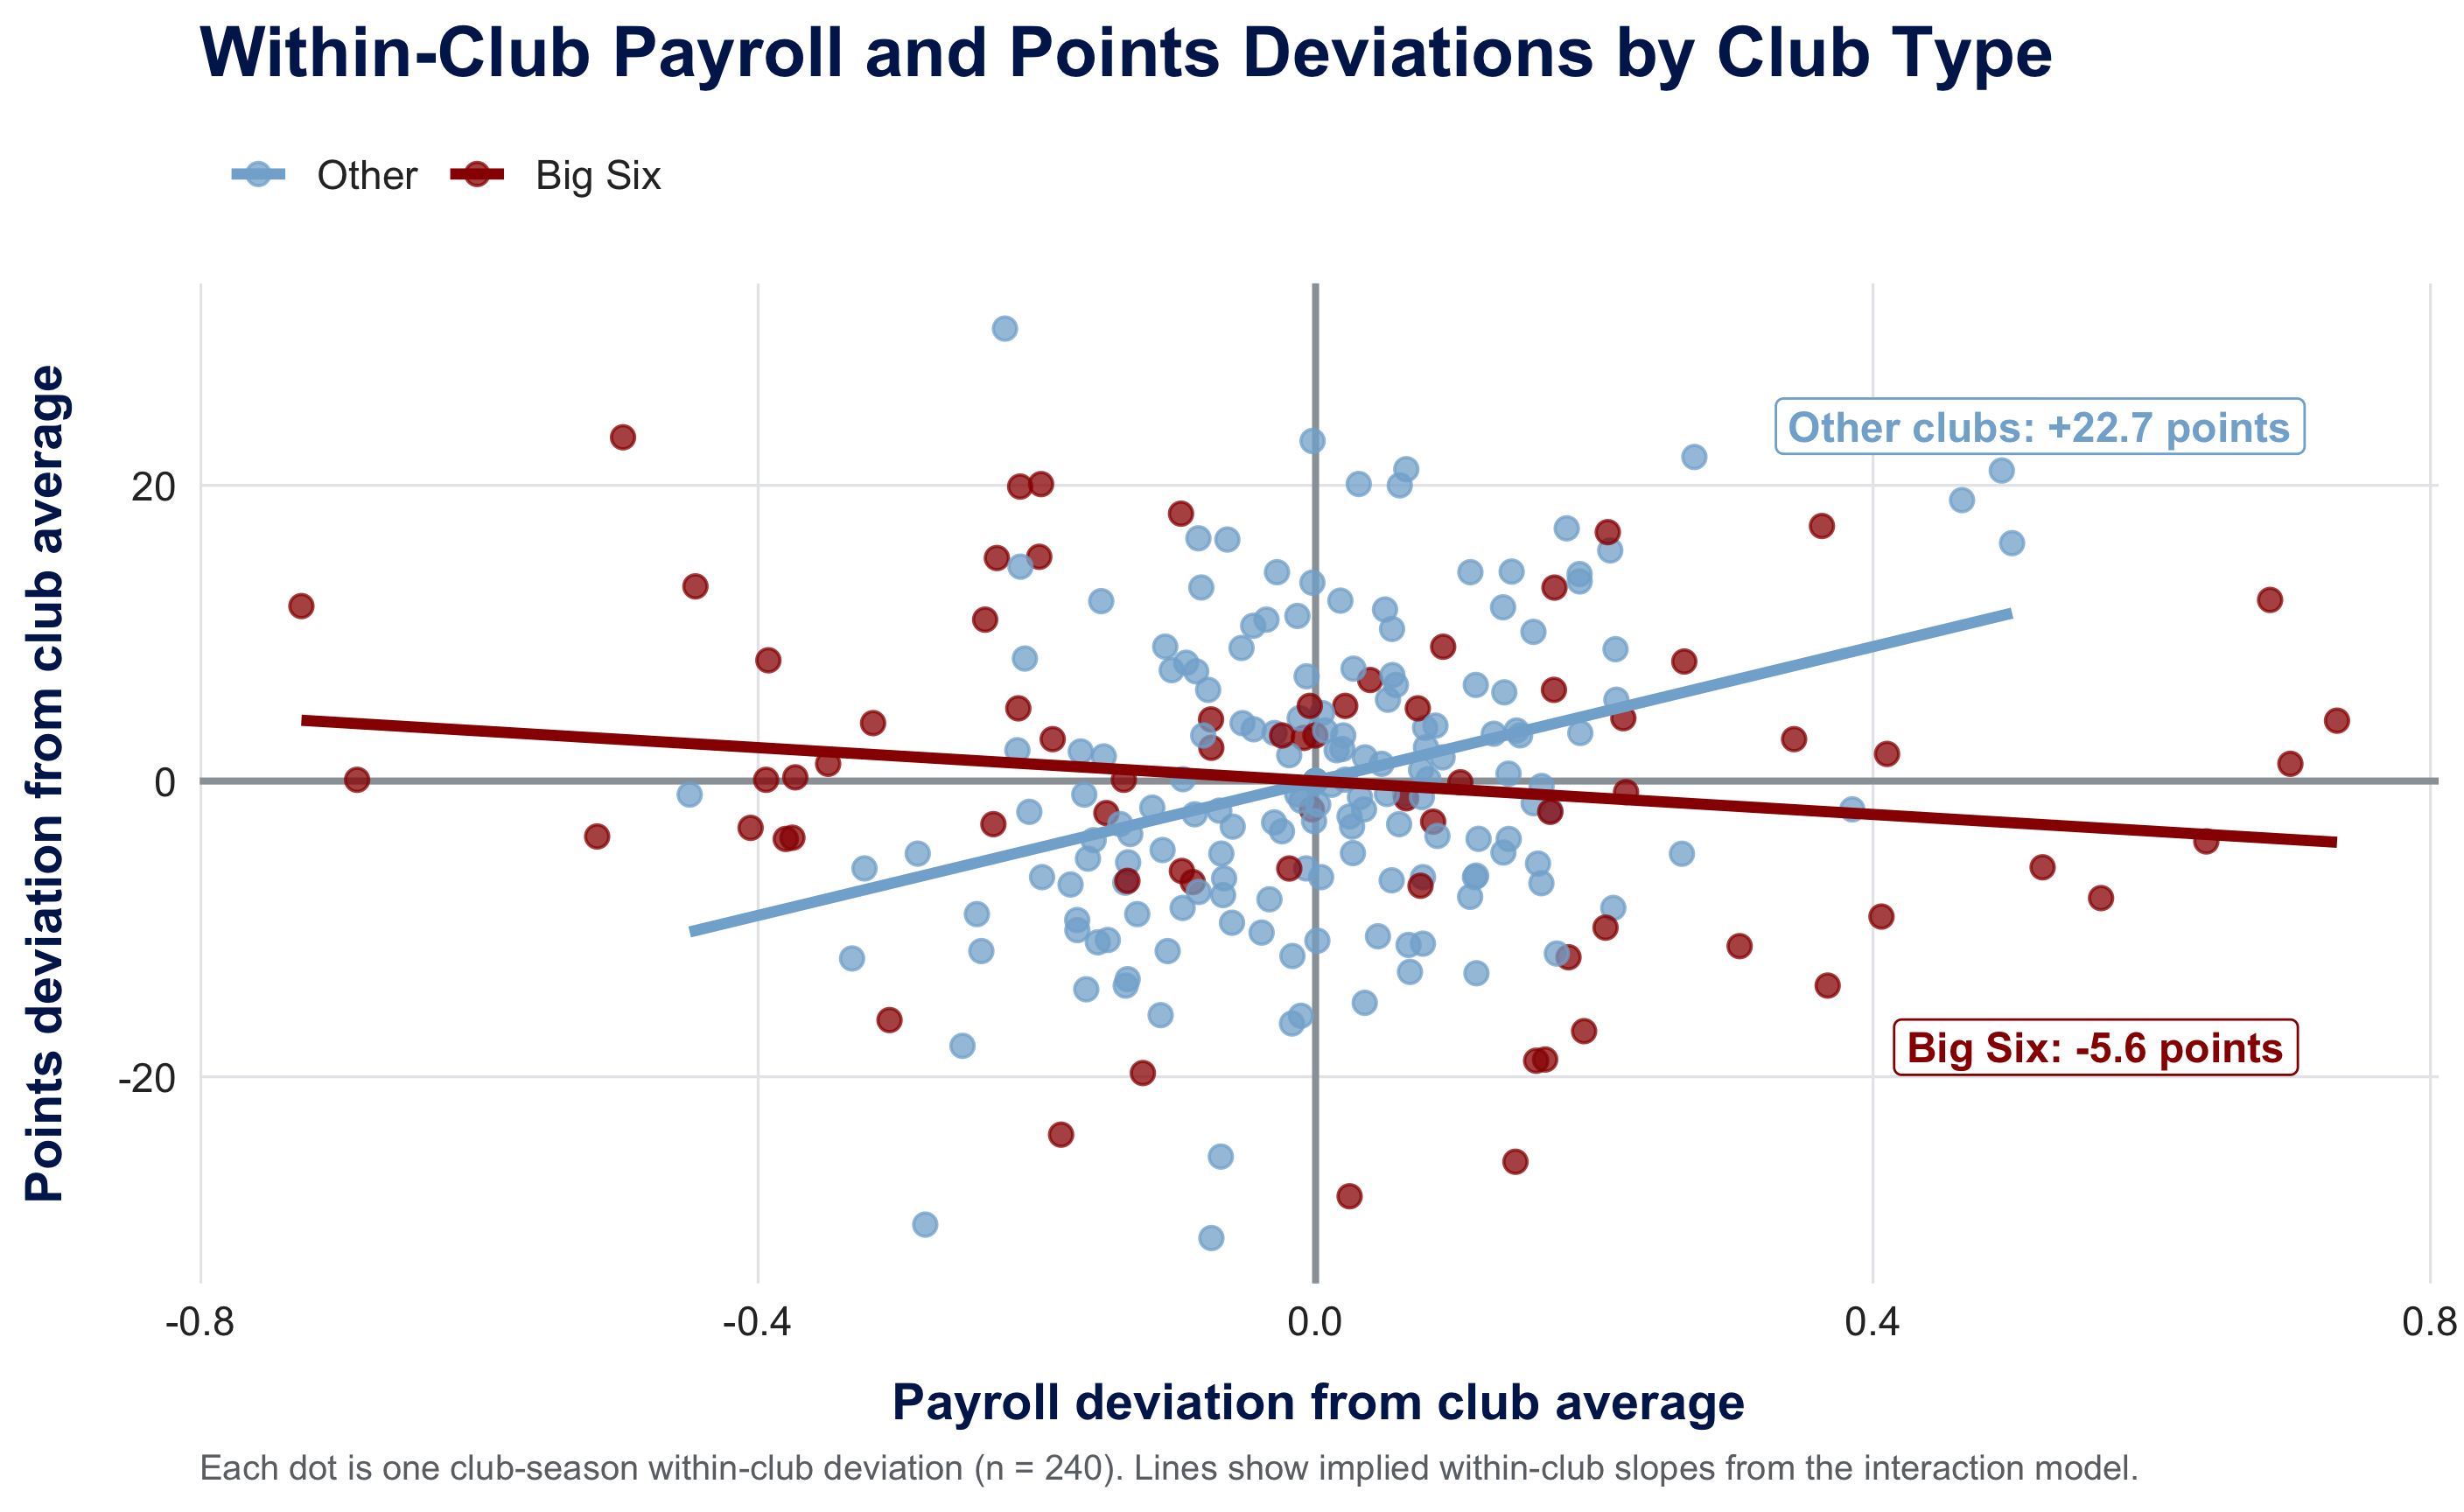
\includegraphics[width=\textwidth]{03_big_six_interaction.png}
\caption*{\textbf{Payroll returns differ sharply by club type.} Each dot is a within-club deviation from that club's average payroll and points (\(n=240\)). The interaction model implies a steep positive within-club payroll slope for non--Big-Six clubs, but a flat-to-negative and statistically unclear slope for Big Six clubs.}
\end{figure}

Payroll therefore looks less like a universal points machine and more like a ladder. It appears most valuable for clubs trying to climb into a higher competitive tier, not for clubs already operating at the top of the market.

For clubs outside the elite tier, the mechanism is intuitive: higher wages can expand the pool of players a club can realistically attract and keep. At the top, the problem changes. The next upgrade is rarer, the bidding is more competitive, and some of the extra payroll may simply be the cost of holding an already-elite squad together.

\section{The Results in One Table}

\begin{table}[H]
\centering
\caption*{\textbf{Payroll matters most outside the Big Six}}
\resizebox{\textwidth}{!}{
\begin{tabular}{llccc}
\toprule
\textbf{Model} & \textbf{Coefficient} & \textbf{Estimate} & \textbf{p-value} & \textbf{Plain-English interpretation} \\
\midrule
Pooled linear & Relative wage bill & 18.20 & $<0.001$ & Strong league-wide association \\
Club fixed effects & Relative wage bill & 3.69 & 0.280 & Weak average within-club association \\
Interaction model & Non--Big-Six wage slope & 22.72 & $9.8\times 10^{-5}$ & Strong positive non--Big-Six association \\
Interaction model & Big Six interaction & $-28.37$ & $6.9\times 10^{-5}$ & Big Six slope is much flatter \\
Interaction model & Implied Big Six wage slope & $-5.65$ & -- & No clear Big Six wage return \\
\bottomrule
\end{tabular}
}
\end{table}

\section{What This Means for Owners}

For owners, the lesson is not ``spend less.'' It is ``know where spending is likely to matter.''

For non--Big-Six clubs, wage spending appears to remain a meaningful competitive lever. A higher payroll can help move a club away from relegation risk, stabilize it in mid-table, or push it toward European qualification. This is the part of the league where a larger wage bill may still buy visible improvement.

For Big Six clubs, the evidence points in a different direction. These clubs already operate near the top of the player market. Additional payroll may be necessary to maintain status, keep stars, and avoid decline, but it does not reliably translate into more league points.

That distinction matters for prospective buyers. An elite club may offer global brand value, commercial revenue, and prestige. But if the objective is to turn new wage investment into visible league improvement, the steeper marginal return may lie outside the Big Six.

In other words, the best payroll investment opportunity may not be the club that already spends the most. It may be the club still close enough to the middle of the market that extra spending can change the caliber of player it can attract.

\section{Payroll Is a Lever, Not a Strategy}

None of this means clubs should treat payroll as an automatic points machine.

Wage spending only matters if it is allocated well. Clubs still need to identify players who fit the squad, avoid overpaying for name value, manage injuries, build strong coaching environments, and decide when non-player investments may have higher returns than another wage increase.

Those non-player investments can include analytics, recruitment infrastructure, medical staff, facilities, academy development, and coaching. A club that spends more without improving how it spends can still waste money.

The fixed-effect results are a warning against the simplest version of the spending story. The average within-club payroll effect is weak. The interaction results sharpen that warning: payroll appears most productive for clubs outside the entrenched elite, but even there, the model estimates an association, not a guarantee.

\section{What This Analysis Can and Cannot Say}

This analysis is observational. Clubs do not choose payroll randomly. Wage bills may respond to expected performance, promotion risk, European qualification, injuries, revenue shocks, or ownership changes. Club fixed effects reduce some confounding by comparing clubs to themselves, but they do not establish causality.

Payroll is also only one dimension of squad investment. Transfer fees, contract length, bonuses, academy production, loan markets, and amortization rules all affect squad quality but are not fully captured by annual wages. A richer financial dataset would allow a fuller view of how clubs convert money into points.

Timing also matters. Wage spending may affect performance with a lag, especially when clubs sign younger players or restructure squads over several windows. A single-season model may miss some of those dynamics.

Finally, Big Six status is a coarse split. It captures a real structural divide in the Premier League, but there is meaningful variation within both groups. Future work could replace the binary classification with a dynamic measure based on revenue, squad value, European participation, wage rank, or club-specific market position.

\section{The Bottom Line}

The Premier League wage table tells a familiar story: richer clubs usually finish higher. But that pattern does not answer the question owners actually face: what happens when a club spends more?

Once we compare clubs to themselves, the average payroll effect becomes much weaker. Then, when we split the league into Big Six and non--Big-Six clubs, the pattern becomes clearer: payroll appears to have its strongest relationship with points outside the elite tier.

For clubs still climbing the talent ladder, higher wages can be a powerful lever. For clubs already at the top, spending more may be less about buying extra points and more about paying the cost of staying there.

\section{Acknowledgments}

The authors would like to thank Professor Adi Wyner and the Wharton Sports Research Seminar for helpful feedback, and the Wharton Sports Analytics \& Business Initiative for supporting this work. All data and code to reproduce this analysis are available at \href{https://github.com/whartonsabi/epl-payroll}{https://github.com/whartonsabi/epl-payroll}.

\end{document}
